% !TEX program = lualatex
% !BIB program = biber
\documentclass[english,aspectratio=43,t]{beamer}
% useful options:
%   aspectratio=169

\usepackage[utf8]{inputenc}
\usepackage{babel}
\usepackage{fixltx2e}
\usepackage{graphicx}
\usepackage{longtable}
\usepackage{float}
\usepackage{wrapfig}
\usepackage{soul}
\usepackage{textcomp}
\usepackage{marvosym}
\usepackage{wasysym}
\usepackage{latexsym}
\usepackage{amssymb}
\usepackage{hyperref}
\tolerance=1000
\usepackage{listings}
\usepackage[iso]{isodate}
\usepackage[backend=biber]{biblatex}

\addbibresource{../src/references.bib}

\definecolor{codegreen}{rgb}{0,0.6,0}
\definecolor{codegray}{rgb}{0.5,0.5,0.5}
\definecolor{codepurple}{rgb}{0.58,0,0.82}
\definecolor{backcolour}{rgb}{1,1,1}

\lstdefinestyle{mystyle}{
    backgroundcolor=\color{backcolour},
    commentstyle=\color{codegreen},
    keywordstyle=\color{magenta},
    numberstyle=\tiny\color{codegray},
    stringstyle=\color{codepurple},
    basicstyle=\ttfamily\footnotesize,
    breakatwhitespace=false,
    breaklines=true,
    captionpos=b,
    keepspaces=true,
    numbers=left,
    numbersep=5pt,
    showspaces=false,
    showstringspaces=false,
    showtabs=false,
    tabsize=2,
    frame=single,
    xleftmargin=2em,
    framexleftmargin=1.57em,
    framexrightmargin=-0.5em
}

\lstset{style=mystyle}
% select theme before using any of its features
\usetheme{Comsys}


\title[Cool]{Finding Concurrency Bugs in Production}
\author{Marvin Strangfeld}
\authorextra{Advisor: Julian Büning}
\subtitle{An Analysis of real-world Techniques}
\date{\today}
\location{Aachen}
%\logoextra{logos/rwth_comsys_cropped}

%\begin{titlepicture}
%	\includegraphics[width=3cm]{images/presentation}
%\end{titlepicture}

\begin{document}


\titleframe


\begin{frame}
	\frametitle{Outline}
	\tableofcontents
\end{frame}


\section{Introduction}
\frame\sectionpage

\begin{frame}[c]{The Danger of Concurrency Bugs}
    \centering
    \begin{block}{Therac-25}
        \begin{itemize}
            \item Computer-controlled radiation therapy machine
            \item Two modes of radiation therapy
            \item Depending on software safety checks that only the intended mode is activated
            \item Race condition between the control and interface task
            \item Three people died because of a radiation overdose
        \end{itemize}
    \end{block}
    % \begin{block}{Northeast blackout of 2003}
    %     \begin{itemize}
    %         \item Power outage throughout parts of the Northeastern and Midwestern United States
    %         \item Race condition in the energy management system
    %     \end{itemize}
    % \end{block}
\end{frame}

\note[itemize]{
    \item Some Test
}

\begin{frame}{Motivation}
    \begin{itemize}
        \item<1-> Parallelism is necessary to achieve high performance on multi-core architectures
        \item<2-> Paths of execution (Threads) are executed mostly non-deterministic
        \item<3-> Heisenbugs -- Bugs that only occur within specific thread interleavings
        \item<4-> \Rightarrow{} Concurrency bugs are not easily reproducible
    \end{itemize}
    \begin{exampleblock}{Goals}<5->
        \begin{enumerate}
            \item Finding concurrency bugs effectively with a minimum overhead of work and computational resources
            \item Preventing concurrency bugs to get into production
        \end{enumerate}
    \end{exampleblock}
\end{frame}

\section{Types of Concurrency Bugs}
\frame\sectionpage

\begin{frame}{Taxonomy of Concurrency Bugs}
    \begin{figure}
        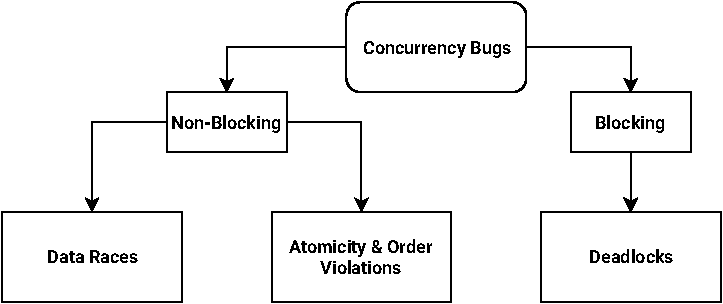
\includegraphics[width=\linewidth]{../src/figures/ConcurrencyBugClasses.pdf}
        \caption{A Taxonomy of Concurrency Bugs -- based on\cite{tchamgoue2012testing}}
    \end{figure}
\end{frame}

\begin{frame}[fragile]{Deadlocks}
\begin{itemize}
    \item Circular dependencies between resources / threads block the flow of the program
\end{itemize}
\begin{lstlisting}[language=Go]
func main() {
    data := make(chan int)
    done := make(chan bool)
    data <- 1 // Program already blocks here
    go func() {
        process(<-data)
        done <- true
    }()
    <-done
}
\end{lstlisting}
\end{frame}

\begin{frame}[fragile]{Data Races}
\begin{itemize}
    \item<1-> Multiple threads simultaneously try to access a shared variable where at least one access is a write operation~\cite{serebry2009threadsanitizer}
\end{itemize}
\begin{lstlisting}[language=Go]<1->
func main() {
	data := make(map[string]string)
	done := make(chan bool)
	go func() {
		data["1"] = "a" // First conflicting access.
		done <- true
	}()
	data["2"] = "b" // Second conflicting access.
	<-done
}
\end{lstlisting}
\begin{itemize}
    \item<2-> Semantical data races
\end{itemize}
\end{frame}

\begin{frame}[fragile]{Atomicity and Order Violations}
\begin{itemize}
    \item Interleaving of threads violate the programmer's intention of atomicity and order
\end{itemize}
\begin{lstlisting}[language=Go]
func main() {
    var group sync.WaitGroup
    group.Add(10)
    sum := 0
    for i = 0; i < 10; i++ {
        go func() {
            sum++ // Not atomic
            group.Done()
        }()
    }
    group.Wait()
}
\end{lstlisting}
\end{frame}

\section{Debugging Techniques}
\subsection{Dynamic Code Analysis}
\frame\sectionpage

\begin{frame}{Record and Replay}
    \begin{block}{Idea}<1->
        Recording the exact path of execution so it can be replayed deterministically
    \end{block}
    \begin{itemize}
        \item<2-> Record
        \begin{itemize}
            \item Thread-Schedule of the program
            \item Non-deterministic variables
            \item External sources of non-determinism (e.g. network traffic)
        \end{itemize}
        \item<3-> Sparse recording~\cite{lidbury2019sparse}
        \begin{itemize}
            \item Selectively ignoring unimportant sources of non-determinism
        \end{itemize}
        \item<4-> \emph{rr} by Mozilla~\cite{mozillarr}
        \begin{itemize}
            \item Can be used with native programs written in any language
            \item No instrumentation needed \Rightarrow{} less perturbation
            \item Runs on stock Linux kernels without system modification
            \item Emulates a single-core machine
            \item Overhead depends on the workload
        \end{itemize}
    \end{itemize}
\end{frame}

\begin{frame}{Data Race Detection}
    \begin{block}{Idea}<1->
        Track program execution to find data races during runtime
    \end{block}
    \begin{itemize}
        \item<2-> \emph{ThreadSanitizer} v2 by Google~\cite{threadSanitizer}
        \begin{itemize}
            \item Build into the Go compiler tool-chain
            \item Compile-time instrumentation of accesses to shared locations
            \item Dynamic annotations to understand the synchronization primitives
            \item Report of potential races based on a state-machine algorithm
        \end{itemize}
        \item<3-> Overhead
        \begin{itemize}
            \item Memory: 5-10x
            \item Execution time: 2-20x
        \end{itemize}
    \end{itemize}
\end{frame}

\begin{frame}[c]{Dynamic Code Analysis}
    \centering
    \begin{exampleblock}{Advantages}
        \begin{itemize}
            \item Easy to use
            \item Could be deployed to production
            \item Can be combined with other debugging tools
        \end{itemize}
    \end{exampleblock}
    \begin{alertblock}{Disadvantages}
        \begin{itemize}
            \item Overhead during execution time
            \item Coverage is quite small
            \item Cannot prevent concurrency bugs to get into production
        \end{itemize}
    \end{alertblock}
\end{frame}

\subsection{Concurrency-aware Testing}
\frame\sectionpage

\begin{frame}{Concurrency-aware Testing}
    \begin{block}{Idea}<1->
        Testing the program for concurrency bugs before it gets deployed into production
    \end{block}
    \begin{itemize}
        \item<2-> Traditional testing mostly covers errors in sequential programs~\cite{lu2008mistakes}
        \item<3-> DEJAVU~\cite{acm2002}
        \begin{itemize}
            \item For the Jalapeno JVM
            \item Using record and replay and delta debugging
            \item Going back and forth between working and failing thread schedules
            \item Narrowing down the failure-inducing thread switch
        \end{itemize}
    \end{itemize}
\end{frame}

\begin{frame}
\begin{figure}
    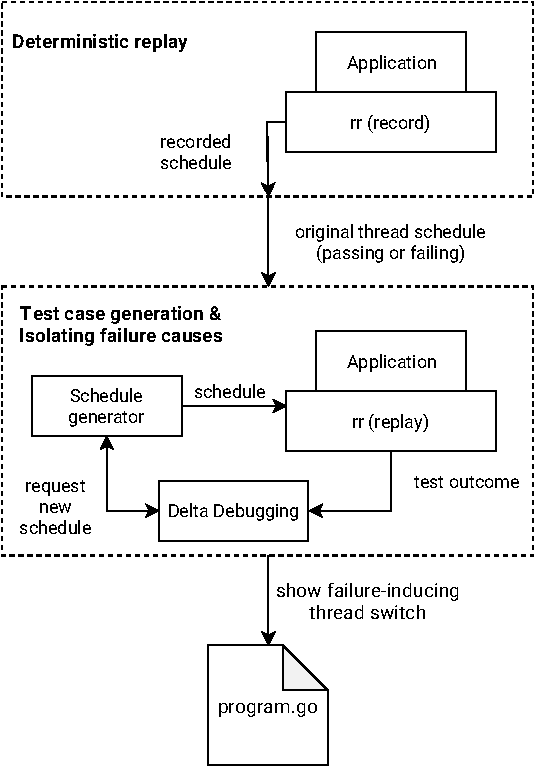
\includegraphics[height=\textheight]{../src/figures/Concurrency-Testing.pdf}
\end{figure}
\end{frame}

\begin{frame}[c]{Concurrency-aware Testing}
    \centering
    \begin{exampleblock}{Advantages}
        \begin{itemize}
            \item Finding concurrency bugs automatically
            \item Can prevent concurrency bugs to get into production
        \end{itemize}
    \end{exampleblock}
    \begin{alertblock}{Disadvantages}
        \begin{itemize}
            \item Operational overhead for setting up the system
            \item Testing time can grow exponentially with the number of threads
            \item Coverage depends on the quality of the tests (semantical correctness)
        \end{itemize}
    \end{alertblock}
\end{frame}

\subsection{Static Code Analysis}
\frame\sectionpage

\begin{frame}{Static Code Analysis}
    \begin{block}{Idea}<1->
        Finding concurrency bugs during compile time by statically analyzing the program
    \end{block}
    \begin{itemize}
        \item<2-> Translating the source code into mathematical models that can be checked
        \item<3-> Mostly infeasible for detecting data races due to the large number of possible thread interleavings
        \item<4-> \emph{Godel Checker}~\cite{godelChecker}
        \begin{itemize}
            \item Static deadlock detector for Go
            \item Converts program code to single static assignments
            \item These can be analyzed by classic model and termination checkers
        \end{itemize}
    \end{itemize}
\end{frame}

\begin{frame}[c]{Static Code Analysis}
    \centering
    \begin{exampleblock}{Advantages}
        \begin{itemize}
            \item Finding concurrency bugs at compile time
            \item Can prevent concurrency bugs to get into production
        \end{itemize}
    \end{exampleblock}
    \begin{alertblock}{Disadvantages}
        \begin{itemize}
            \item Takes a lot of time to check
            \item Only feasible for programs with little parallelism
        \end{itemize}
    \end{alertblock}
\end{frame}

\section{Conclusion}
\frame\sectionpage

\begin{frame}{Conclusion}
    \begin{itemize}
        \item<1-> Dynamic Code Analysis
        \begin{itemize}
            \item Record and replay can be used to deterministically reproduce bugs
            \item Dynamic data race detection can be used to find data races at runtime
            \item \textbf{Advantage:} Easy to use and easy to deploy
            \item \textbf{Disadvantage:} Large overhead and small coverage
        \end{itemize}
        \item<2-> Concurrency-aware Testing
        \begin{itemize}
            \item Testing different thread schedules for concurrency bugs
            \item \textbf{Advantage:} Prevent concurrency bugs to get into production
            \item \textbf{Disadvantage:} Operational overhead of setting up and maintaining the system and tests
        \end{itemize}
        \item<3-> Static Code Analysis
        \begin{itemize}
            \item Translate code into mathematical models to check correctness
            \item \textbf{Advantage:} Find concurrency bugs at compile time
            \item \textbf{Disadvantage:} Only feasible for applications with little parallelism
        \end{itemize}
    \end{itemize}
\end{frame}

\begin{frame}[noframenumbering,plain,allowframebreaks]{Sources}
    \printbibliography[heading=none]
\end{frame}

\end{document}
